\documentclass[main.tex]{subfiles}

\begin{document}

\section{Configuration System}
\label{section: configuration}
\textit{This section goes over the general requirements of a configuration system for the pCT project and how it is implemented. It will go over the GUI designed for the configuration and its functionality, along with the API it uses to receive and transmit data. Next, a database solution is presented, using MongoDB to store configuration sets; lastly, a ramp-up algorithm is described and implemented that is to be used in the powering-on sequence of the \gls{dtc}.}


 Seven registers on the microcontroller determine the threshold values for DVDD, AVDD, PWELL, and temperature. The configuration system must be able to configure the threshold registers quickly, and use the enable signals to power on the strings.

Each layer can have different nominal threshold values for voltage and current and therefore it is necessary to be able to change these values as we test the strings. A complete set of threshold values for all strings in every layer of the \gls{dtc} will be referred to as a configuration set. The configuration sets must be stored in a database, and MongoDB was chosen for storing the sets; we will discuss the database more in \autoref{ssec: mongo}.

All this leads to a requirement for a user-friendly configuration system that can configure the microcontrollers through IPbus, store configuration sets, and power on the \gls{dtc}. Furthermore, these parts must be developed modular and generic to make the system scalable and easy to modify.

\subsection{Configuration API}
\label{ssec: mcu_api}
IPbus sends and retrieves information between the control software and the MB Hub. IPbus has a software library, $\mu$HAL, that provides end-user API for C++ and Python. For this project, Python is used to interface with uHAL and IPbus. This \gls{api} can issue read and write commands to the IPbus module on the MB Hub and dispatch these commands in a single packet. Subsection \ref{ssec: IPbus} provides a detailed discussion of the IPbus software and how to implement it in Python. $\mu$HAL allows us to send and receive data, but this \gls{api} is not sufficient for communicating with the microcontroller; there must be an additional interface that has functions for our FPGA design, and the microcontroller on the \gls{mb}. Following the principles of \gls{oop}, it is natural to encapsulate the properties of the API into two interfaces, one for the MB Hub and one for the microcontroller on the \gls{mb}. Additionally, the configuration system requires several high-level processes to operate, and therefore a separate configuration \gls{api} is required.

\subsubsection{IPbus API}
The IPbus \gls{api} contains functions for read and write commands using uHAL, broadcast functionality using the global module, and enabling/disabling the com\_modules for individual layers. This interface Python class is named "ipbus low interface".

An essential part of the \gls{api} is the "issue" functions. Subsection \ref{ssec: IPbus} discusses how IPbus benefits from packing data in larger payloads before dispatching them, which is the purpose of the "issue" functions. The "issue" functions loads the data request in a payload without sending it to the MB Hub. This can optimize the communication chain between the control software and the microcontroller by limiting the number of network dispatches performed.

\subsubsection{Microcontroller API}

The \gls{api} for the microcontroller must interface with the microcontroller and, by extension, the MB Hub. Therefore, the microcontroller \gls{api} uses the IPbus \gls{api} as a lower-level communication interface. The microcontroller \gls{api} has similar functions as the IPbus \gls{api}, except it uses namedtuples to create the data header for communicating with the microcontroller.

Namedtuples is a container in Python with user-defined parameters. The address map of the microcontroller has been defined in a separate package called \textit{mcu\_addr}. An image of the namedtuple created for the microcontroller \gls{api} is given in \autoref{lst: namedtuple}.

\lstset{frame=tb,
  language=Python,
  aboveskip=3mm,
  belowskip=3mm,
  showstringspaces=false,
  columns=flexible,
  basicstyle={\small\ttfamily},
  numbers=none,
  numberstyle=\tiny\color{gray},
  keywordstyle=\color{blue},
  commentstyle=\color{dkgreen},
  stringstyle=\color{dkgreen},
  breaklines=true,
  breakatwhitespace=true,
  tabsize=3
}


\begin{lstlisting}[caption={Code showing the construction of the namedtuple in the "mcu\_addr" package.},captionpos=b, label=lst: namedtuple]
register_addr = namedtuple('register_addr', ['name','addr_val', 'num_bits', 'measurement_type', 'RW'])
    \end{lstlisting}



The namedtuple contain information such as name, address value, number of bits, measurement type, and read/write access of a register. The \gls{api} retrieves information from the namedtuple and uses it to communicate with the microcontroller. This serves two purposes, first, the user does not need to know the address map of the microcontroller; they only enter the name of a namedtuple, and the \gls{api} takes care of the rest. Second, the \textit{mcu\_addr} package is a common access point for the microcontroller address map. If a developer in the future needs to add a register, or change the address value of an existing register, then one only needs to edit a single file, the \textit{mcu\_addr} package.


\subsubsection{Configuration API}
\label{ssec: conf_api}
The configuration process requires several functions to load configuration sets from the database, verify handshake values from the MB Hub, and configure the relevant registers on the \gls{mb}. A top-level \gls{api} has been created for this purpose, and a diagram of the interface hierarchy for the configuration system is given in \autoref{fig: interface_hierarchy}.


\begin{figure}[!ht]
    \centering
    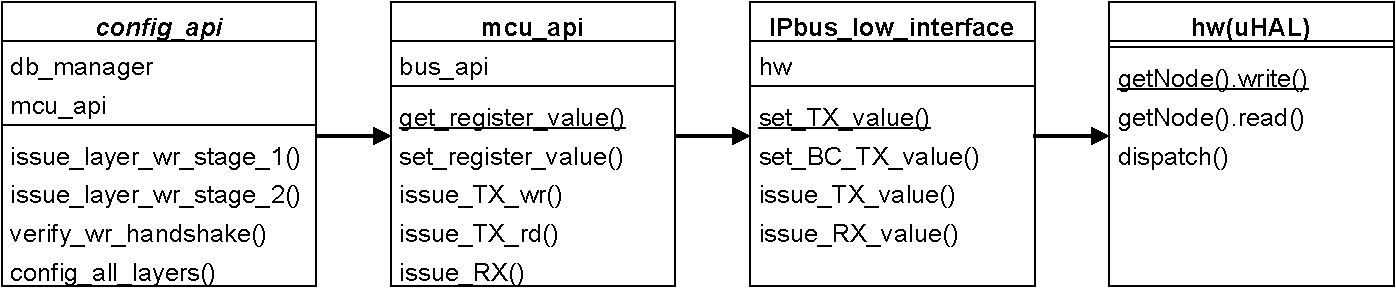
\includegraphics[width=15cm, scale=4]{images/interface_hierarchy.pdf}
    \caption{Interface hierarchy for the configuration system.}
    \label{fig: interface_hierarchy}
\end{figure}
\FloatBarrier

The "\textit{config\_api}" class contains a "db\_manager" object and an "mcu\_api" object; they handle database operations and communicate with the microcontroller, respectively. Setting up the configuration system only requires the user to instantiate a \textit{config\_api} object in a python script. This class \gls{api} has several functions for verifying handshakes, retrieving data from the database, and performing the ramp-up process. \textit{config\_api} has two functions for issuing configuration commands down to the \gls{dtc}, stage 1 and stage 2. These two will be discussed more in \autoref{ssec: power_algo}. The \textit{config\_online\_layers}-function is the main function of the \gls{api} that performs the entire configuration process.



\subsection{Powering algorithm}
\label{ssec: power_algo}
There are several procedures and constraints for powering and configuring the strings of the DTC. Tasks such as enabling layers, sending configuration data and verifying handshakes must be performed every time the system is turned on. The calorimeter is made of 43$\cdot$12 strings that all consume a significant amount of current. Several constraints must be considered while powering on such a system. Powering on all strings at once could cause a high inrush current that could cause a system malfunction if handled incorrectly. A solution to this is to develop a ramp-up algorithm that turns on each string one by one, gradually increasing the power level of the strings. 

The algorithm must perform these tasks:

\begin{itemize}
    \item Get the configuration values from the database.
    \item send write requests to every layer.
    \item verify handshake values from the write requests.
    \item Turn on each string and set threshold levels sequentially, and verify they do not get turned off by the microcontroller. This is to limit the current consumption of the strings while turning them on.
\end{itemize}

The configuration \gls{api} contains functions that perform handshakes, and stages write commands to IPbus, and the \textit{config\_online\_layers}-function wraps these together to perform the configuration. The stage 1 and 2 functions are responsible for retrieving the values from the database and issuing the write requests for the specified layer. Stage 1 issues the write requests for the threshold 1 registers with static values; stage 2 handles the threshold 2 registers, and turns on the strings sequentially.

The reasoning behind having two stages is twofold, to prevent unnecessary write operations and to ensure more readable, concise code. Only four of the eight registers need to be changed when a new string is turned on, the three threshold values for AVDD, DVDD and PWELL, and the enable signal, which turns on the next string. If a single function issued all the write requests, we would have to configure twice as many registers each time a string turned on. Stage 1 issues the write requests for the four static registers during the ramp-up process, while stage 2 issues requests to the four registers that change for each string. It is important to note that the global module is not used for the configuration process. The layers are assumed to have different threshold levels, so they are configured individually.

The algorithm will first use stage 1 to configure all layers, then use the stage 2 function in a loop, to gradually turn on the strings and set appropriate threshold levels. A flowchart configuring one layer is given in \autoref{fig: flow_chart}.

\begin{figure}[!ht]
    \centering
    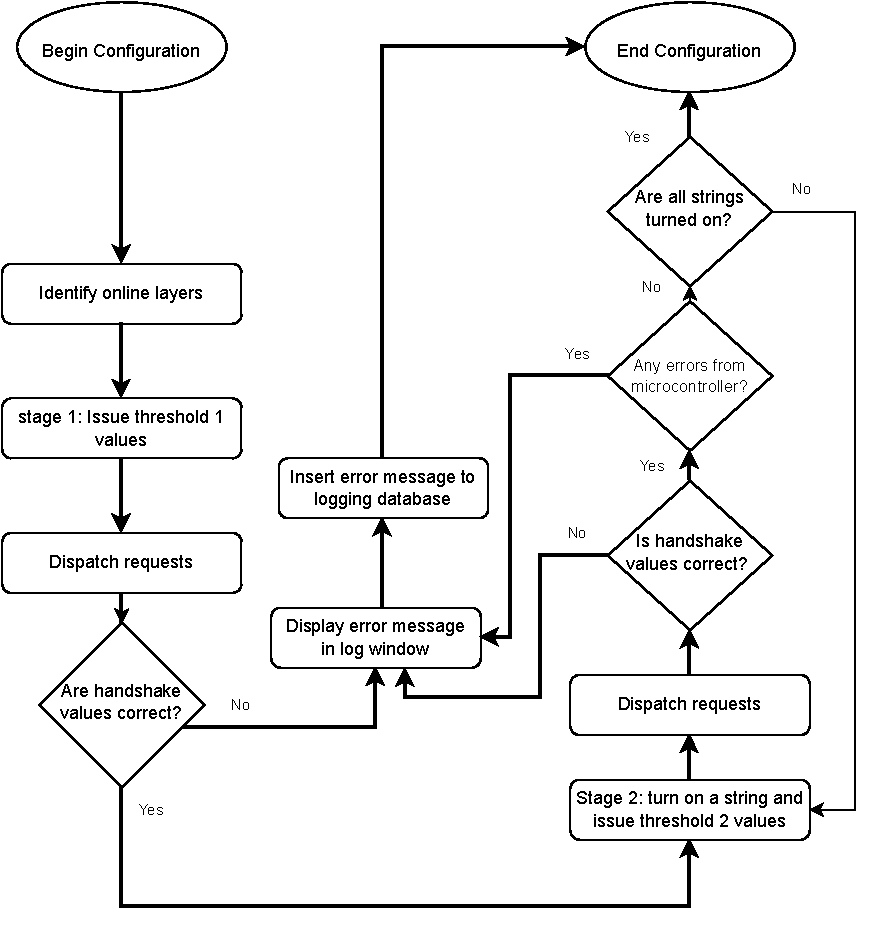
\includegraphics[width=12cm, scale=1.5]{images/Configuration Flowchart.pdf}
    \caption{Flowchart of the configuration function of a single layer.}
    \label{fig: flow_chart}
\end{figure}
\FloatBarrier

The function loops through all online layers during stage 1 and 2. The flowchart describes how one layer is configured during the function.

The left side of \autoref{fig: flow_chart} shows the flowchart of stage 1, where the warning threshold levels are set, along with the temperature limit. All the commands are issued prior to being dispatched as a single packet. Finally, the handshakes are verified. The right side of the figure shows stage 2, where it turns on the strings individually. The \textit{error count} register from the microcontroller is checked at the end of the loop to assert whether any strings were turned off due to high currents. 

The flowchart checks for errors during configuration, but the error handling afterwards has yet to be fully implemented. Ideally, the error messages should be displayed to the user and also be logged in a database, including a severity grade of the error.


\subsection{MongoDB Database}
\label{ssec: mongo}
The database chosen for the configuration is MongoDB. MongoDB was chosen because it is a popular, open-source, NoSQL database with Python API libraries. In addition, MongoDB is capable of storing large amounts of data, which helps store many large configuration sets. The APIs access the database through the \textit{db\_manager} class, which interfaces with the PyMongo library. The configuration of the readout chips also implements MongoDB, and using the same database for both systems reduces the modular complexity of the \gls{pct}-system.

The hierarchy of a MongoDB database is shown in \autoref{fig: mongo_chart}.

\begin{figure}[!ht]
    \centering
    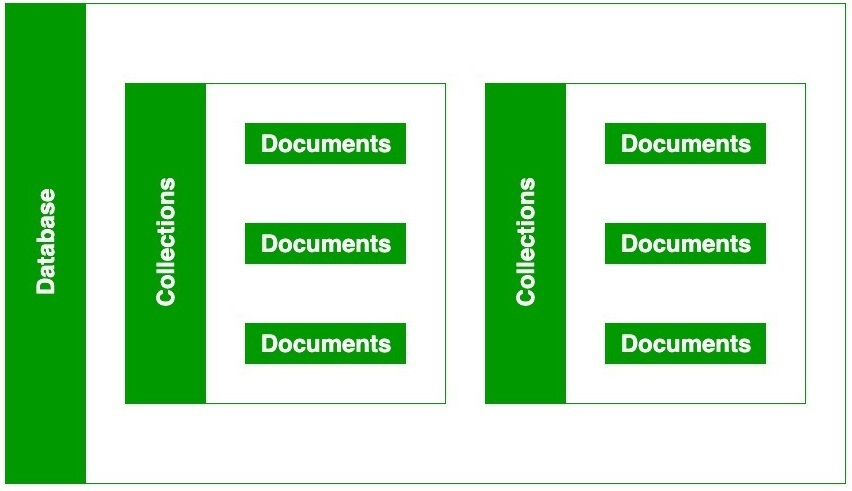
\includegraphics[width=12cm, scale=1.5]{images/mongodb-nosql-working.jpg}
    \caption{Hierarchy of a database in MongoDB.}
    \label{fig: mongo_chart}
\end{figure}
\FloatBarrier

Each database contains user-defined collections that each store their documents. For example, if we used one MongoDB database for both the readout and the power control, we would have one collection for each system.

MongoDB uses JSON as the template for its databases, JSON being a widely used text-based data format for storing and transferring data. A typical example of a MongoDB JSON document is shown below in \autoref{lst: mongo_example}.


\begin{lstlisting}[caption={Example document using JSON to store information.},captionpos=b, label=lst: mongo_example]
{
    "name": "John",
    "age": 22,
    "hobby": {
	"reading" : true,
	"gaming" : false,
	"sport" : "football"
    },
    "class" : ["JavaScript", "HTML", "CSS"]
}
    \end{lstlisting}



A document contains fields, and each field contains a corresponding value. This value can be a number, string, or dictionary of subfields; the "hobby" field in \autoref{lst: mongo_example} contains three fields with their values. For our purpose, the format of the initial configuration set was simple, each field only needed to contain a single value, and each layer required its own set. Each configuration set must also contain a "last updated" timestamp for documentation, and it must have a field for enabling the com\_modules on the \gls{fpga}. Two iterations of the database format were made; the first iteration of this data format is shown in \autoref{lst: json_v1}.

\begin{lstlisting}[caption={First iteration of JSON format of a configuration set.},captionpos=b, label=lst: json_v1]
{
	"_id": {
		"$oid": "6295fd811cb9e58814cbd477"
	},
	"Config name": "Test",
	"Configuration values": [
		{
			"layer": 1,
			"Temperature limit": 111,
			"DVDD threshold 1": 500,
			"AVDD threshold 1": 600,
			"PWELL threshold 1": 700,
			"Enable signals": 4095,
			"DVDD threshold 2": 112,
			"AVDD threshold 2": 150,
			"PWELL threshold 2: 200
		},
    \end{lstlisting}



Each set has a unique name, and the configuration values are stored in dictionaries inside the "configuration values" field. This field contains a separate dictionary for each layer, containing the eight threshold values. Retrieving the information using Python is done by using a "get" command for the threshold values.

One of the challenges behind the ramp-up algorithm is that strings' current consumption can vary depending on the quality of the chips on the string. Some strings can draw double the current compared to others, and implementing this into the ramp-up process would only be possible if we knew each string's threshold values. The second iteration of the database contains individual threshold values for each string to alleviate this current consumption problem. \autoref{lst: json_v2} shows an outline of this database implementation.

\begin{lstlisting}[caption={Second iteration of JSON format of a configuration set, with for individual strings.},captionpos=b, label=lst: json_v2]
{
	"_id": {
		"$oid": "6295fd811cb9e58814cbd477"
	},
	"Config name": "Test",
	"Configuration values": [
		{
			"layer": 1,
			"Temperature limit": 111,
			"DVDD threshold 1": 500,
			"AVDD threshold 1": 600,
			"PWELL threshold 1": 700,
			"Enable signals": 4095,
			"DVDD threshold 2": {
				"String 1": 1,
				"String 2": 4,
				"String 3": 7,
				"String 4": 10,
				"String 5": 6,
				"String 6": 7,
				"String 7": 8,
				"String 8": 9,
				"String 9": 10,
				"String 10": 11,
				"String 11": 12,
				"String 12": 13
			},
    \end{lstlisting}




This new iteration is similar to the first, but all the threshold 2 levels for PWELL, DVDD, and AVDD are dictionary objects containing values for each string. The configuration API must sum these string values while performing the ramp-up process, leading to more logic on the software side, specifically for the configuration \gls{api}.

Setting up the database format and creating new sets is performed with  \textit{db\_manager}. This class contains functions for communicating with the Mongo database, creating new configuration sets and updating these sets with new values. All data formatting happens in this class, the Mongo database does not perform any special functions in manipulating the stored data.



\subsection{Configuration GUI}  
\label{ssec: cgui}
The configuration API contains many functions for setting up the configuration process and managing the Mongo database. However, this class requires an \gls{hmi} that allows for quickly setting up configuration data and is user-friendly. A person with no knowledge of the underlying process behind the configuration must be able to load a configuration set from the database and start the configuration of the strings. A logical answer to this problem is to implement a \gls{gui} for the configuration system. However, unlike the monitoring system, no commercial \gls{gui}s exist that can be applied to our configuration system, and thus a custom-made \gls{gui} must be implemented.

The primary feature the \gls{gui} requires is the ability to load configuration sets from the database and start the configuration with the push of a button. The \gls{gui} must also have an "advanced" tab that allows the user to create new configuration sets directly, insert them into the database, and modify existing sets.

Building the \gls{gui} and designing it is performed using Qt Designer. The Python library, PyQt5 is used to interface the \gls{gui} with our configuration \gls{api} and database. QT Designer was used to design the \gls{gui} because it is easy to work with, and this tool has also been used previously to create GUIs for the readout electronics.


The class chart for the configuration GUI is given in \autoref{fig: gui_chart}.

\begin{figure}[!ht]
    \centering
    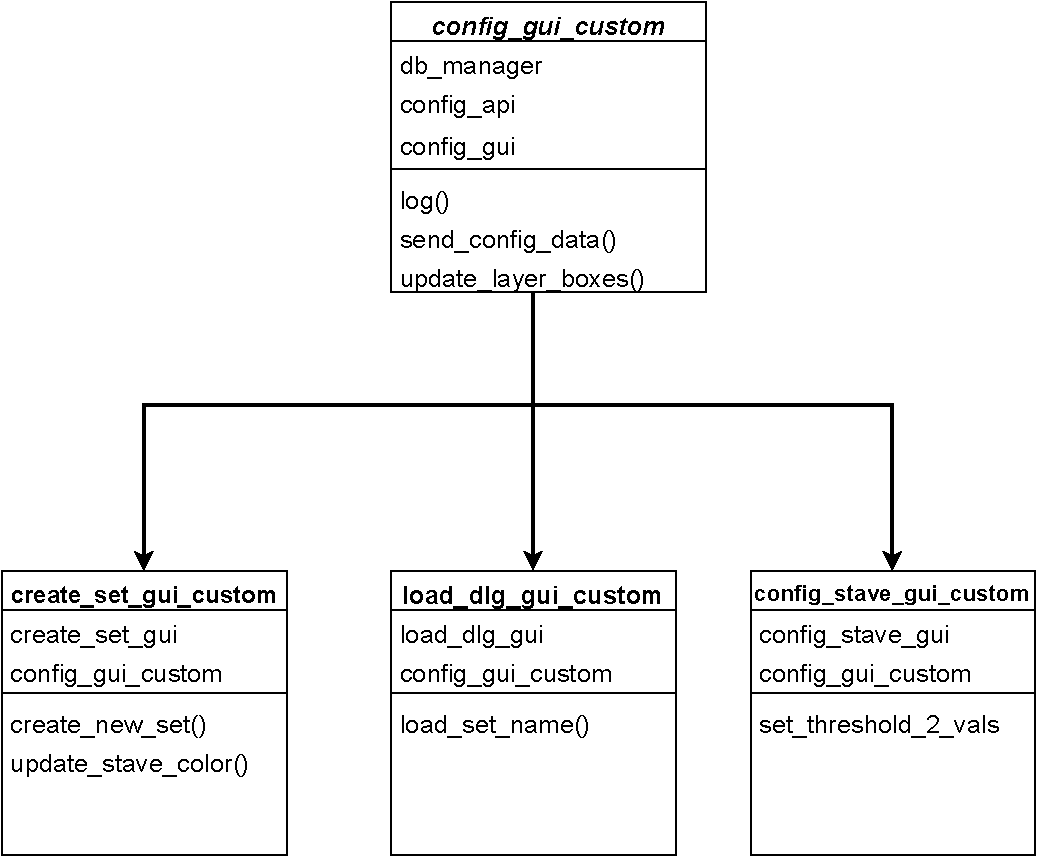
\includegraphics[width=12cm, scale=1.5]{images/gui_class_diagram.pdf}
    \caption{Class diagram of the configuration GUI.}
    \label{fig: gui_chart}
\end{figure}
\FloatBarrier

The GUI is made out of 4 custom Python classes, \textit{config\_gui\_custom} is the main window for the user. The other classes are the windows for creating new configuration sets, loading sets from the database, and setting the individual string threshold values. The \textit{config\_gui\_custom} instantiates the configuration \gls{api} and database manager and connects their functions to the GUI buttons.

The main window of the GUI is shown in \autoref{fig: gui_window}, displaying the "basic" tab.

\begin{figure}[!ht]
    \centering
    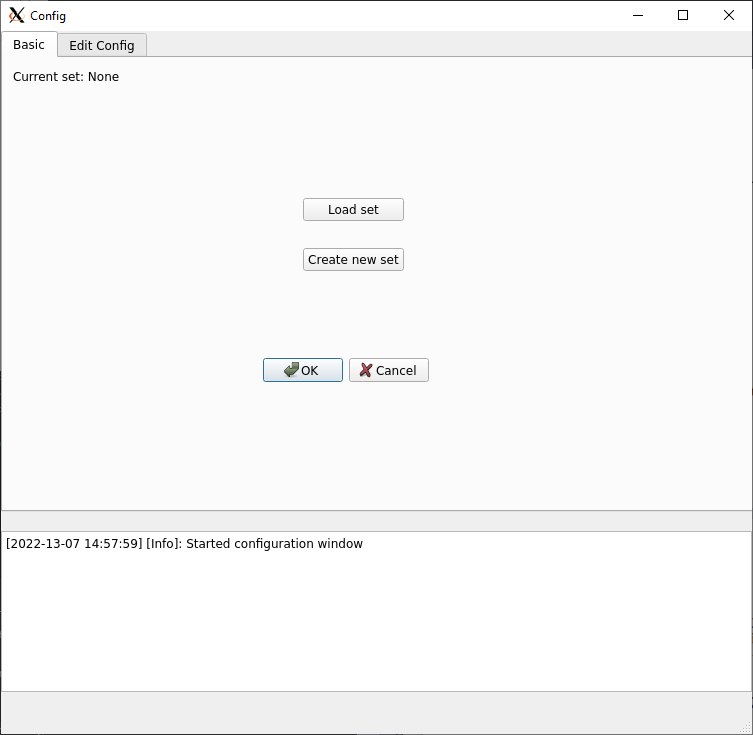
\includegraphics[width=10cm, scale=1.5]{images/gui_main.png}
    \caption{Image of the main window of the configuration GUI.}
    \label{fig: gui_window}
\end{figure}
\FloatBarrier

The window has buttons for loading a set from the database, creating a new set and inserting it into the database, and confirm/cancel dialogue buttons. The upper left of the window shows which configuration set is currently loaded. The window has a log window that informs the user of actions performed, errors, and confirmation messages. These log messages are currently only displayed in the \gls{gui}, since a logging database have yet to be implemented. A typical use case for the "basic" tab is loading a set from the database and then clicking the "start configuration" button on the main hub GUI to start the configuration process.

Clicking the "Load set" button will open up a dialogue window, showing every set in the database.

\begin{figure}[!ht]
    \centering
    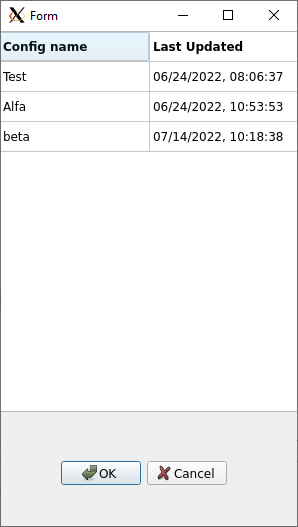
\includegraphics[ scale=0.6]{images/load_dlg_window.png}
    \caption{Image of load set window.}
    \label{fig: load_window}
\end{figure}
\FloatBarrier

As shown in \autoref{fig: load_window}, the window shows every set along with a timestamp of when it was last updated. Choosing a set to load is done by clicking on the set and pressing the "OK" button.

The "Edit Config" tab allows for both reading and modifying the threshold values for each set. It is shown in \autoref{fig: edit_tab_window}.

\begin{figure}[!ht]
    \centering
    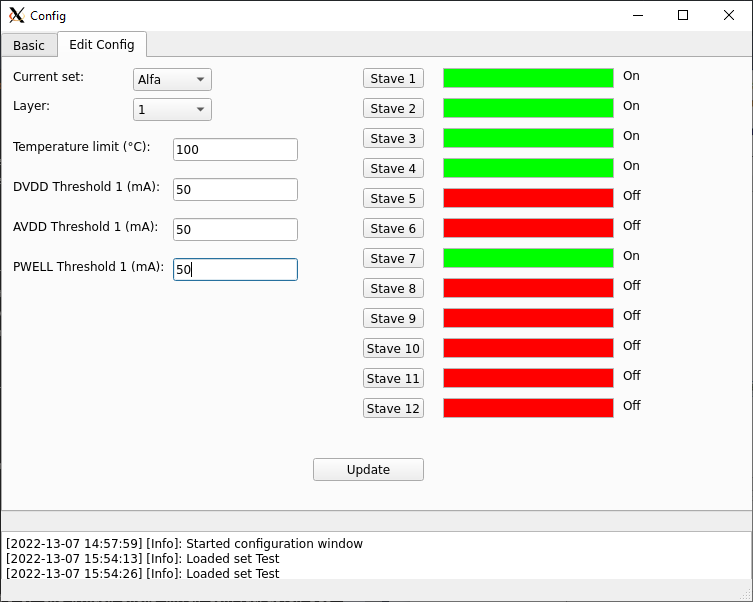
\includegraphics[scale=0.55]{images/config_tab_gui.png}
    \caption{Image of the "Edit Config" tab.}
    \label{fig: edit_tab_window}
\end{figure}
\FloatBarrier

The threshold values can be set for each layer, and enable signals for the strings can be changed interactively by clicking on their corresponding coloured box. The log window will alert the user when changes are made to a configuration set. This tab helps make small changes to existing sets but requires the user to know the structure of the configuration sets to edit them.

The "Create set" button opens a window similar to the "Edit Config" tab, allowing the user to create a new set. The user cannot set different values for each layer while creating it; instead, the "Edit Config" tab can be used afterwards to make edits.


\subsection{Configuration Timing}
\label{ssec: con_timing}

Configuring the layers of the \gls{dtc} requires sending multiple write requests through the \gls{pcs}, which can take a significant time to perform. If the process is slow, it will feel sluggish for the user, impacting the user experience. Additionally, debugging the hardware becomes tedious and unrealistic if the configuration is slow; it is therefore vital to ensure the configuration is as fast as possible. The transmission speed of software, IPbus, MB Hub and microcontroller all affect the configuration process. The configuration should take at most 10 seconds to complete as a benchmark. Any longer and the system will feel sluggish and laggy to the user.

We will first cover the calculated delay of the configuration system. As mentioned in \autoref{ssec: IPbus}, the transmission speed of performing one read/write with IPbus is 250 $\mu$s, but this can be improved per package by sending larger packets at once. The \gls{fpga} is an UltraScale high-speed board with an internal system clock of 300 MHz, meaning each instruction takes approximately 3 ns to perform, which we will assume is negligible compared to the other sources of delay in the \gls{pcs}. The last chain in the \gls{pcs}, the microcontroller on the \gls{mb} can have a maximum baud rate of 1 Mbit/s, leading to 1 $\mu$s transmission speed per bit. Writing to the microcontroller requires sending 32 bits + 1 start bit; this results in a delay of: 

\begin{equation} \label{eqn:mu_calculation}
\frac{n}{\mu_{baud}}=\frac{33}{921600}\approx33 \mu s
\end{equation}

Where n is the number of bits being sent. The calculated delay of one write down to microcontroller becomes:

\begin{equation} \label{eqn:write_delay_equation}
t_{write}+t_{\mu }= 250 + 33 = 288\mu s
\end{equation}

The configuration of the layers is done in parallel; the \gls{fpga} can transmit data to all layers at once, so the configuration timing of one layer will approximately equal the configuration timing of so to calculate delay, we need only look at the configuration timing of a single layer. Eight registers must be written initially; for each string turned on, three threshold registers and the enable signal register must be written. This amounts to 8 + 4$\cdot$12 = 56 write requests for a single layer. Confirming the handshake values must be done individually by software, and performing 56 write requests for 43 layers leads to reading 56*43 handshake values. The theoretical delay for an entire configuration process will then be:

\begin{equation} \label{eqn:total_delay_equation}
2\cdot(56\cdot43)\cdot t_{IPbus}+56\cdot t_{\mu }= 4816 \cdot 250 + 56\cdot33 \approx 1.2 s
\end{equation}

It is important to note that the delay of the software is not considered in this calculation, only the delay through the \gls{pcs} chain. This calculation also considers the worst-case scenario of the IPbus delay being 250 $\mu$s; we can expect the delay from the IPbus to be significantly shorter per data packet sent when sending large data packets at once. We can see from \autoref{eqn:total_delay_equation} that the calculated delay amounts to 1.2 s, which is significantly faster than our maximum of 10s.

\subsubsection{Testing configuration timing}

The next step is to measure the actual delay of the \gls{pcs}. We currently have a prototype layer of the \gls{pcs} running, a communication link from the software to the microcontroller. Only one layer is operational; therefore, tests performed will be incomplete and may not be completely accurate, but it will still give us a rough estimate of the expected delay in the final product. For comparison sake, we will first calculate the estimated configuration timing for one layer using \autoref{eqn:total_delay_equation}:

\begin{equation} \label{eqn:one_layer_delay}
2\cdot(56\cdot1)*\cdot t_{IPbus}+56\cdot t_{\mu }= 112 cdot 250 + 56*33 \approx 30 ms
\end{equation}

We can expect the measurements of the delay to be approximately 30 ms. The test configures the microcontroller 1000 times and calculates the average time and standard deviation. The time measurement is done with the Time library from Python, which includes the software delay of the system, and can lead to minor inaccuracies in the measurements.

The test setup had an average configuration time of 51ms($\sigma$ = 7ms), close to the calculated value but not wholly accurate. This can be explained by the software delay or other small processes in the transmission that were not accounted for in the calculations.

From the test, we can expect the configuration timing of all 43 layers to be slightly larger than the calculated timing from \autoref{eqn:total_delay_equation}.




\end{document}


